\section{Design}
\subsection{Block Diagrams}
The design of this project is modular in nature. It is desired to have one main controller and
multiple remote temperature sensors and vent controllers, as shown in Fig.~\ref{fig:maindiagram}. Fig.~\ref{fig:cntldiagram} will show the main control panel in more detail, while Fig.~\ref{fig:remotediagram} will show the remote temperature sensors, and Fig.~\ref{fig:remotediagram} will show the vent controllers.  Each component will be described in further detail in \S\ref{sect:blockdescriptions}.

\begin{figure}[htb]
\centering
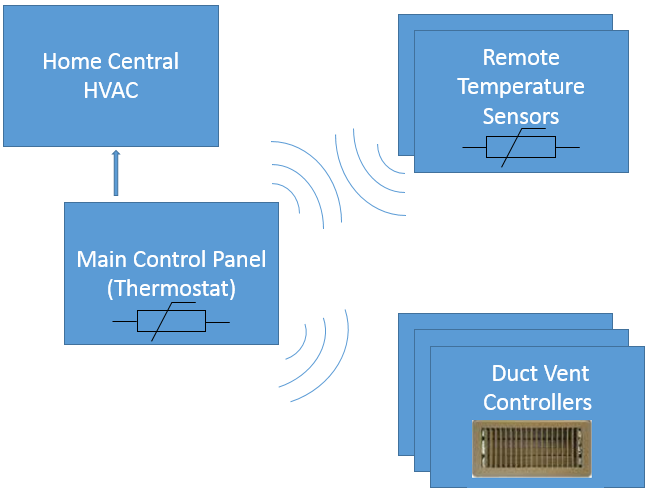
\includegraphics[width=.9\textwidth]{OverallDiagram.png}
\caption{Top level system diagram.}
\label{fig:maindiagram}
\end{figure}

\begin{figure}[htb]
\centering
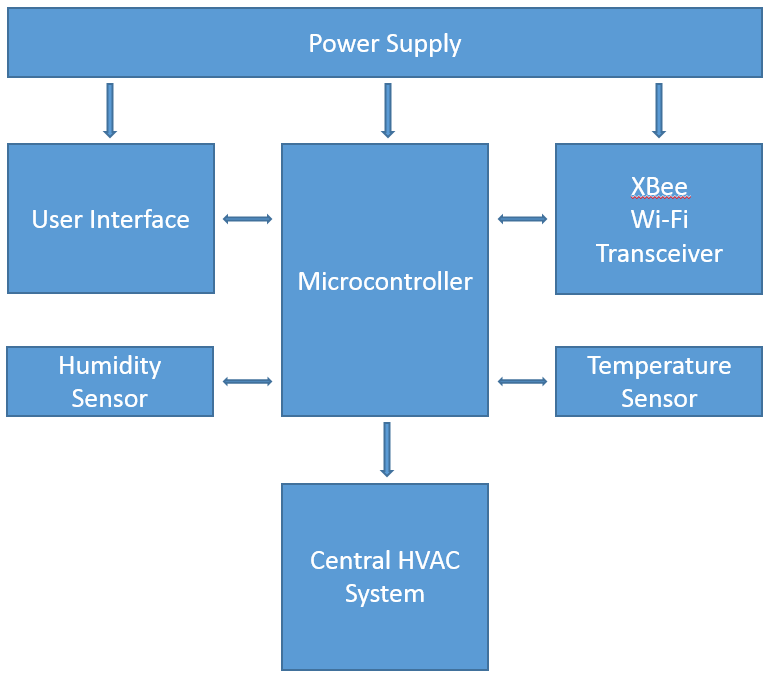
\includegraphics[width=.9\textwidth]{MainCntlBlockDiagram.png}
\caption{Main Control Panel component Diagram from Fig.~\ref{fig:maindiagram}.}
\label{fig:cntldiagram}
\end{figure}

\begin{figure}[htb]
\centering
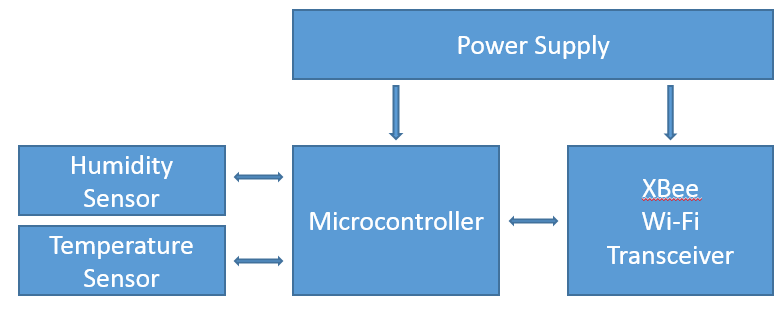
\includegraphics[width=.9\textwidth]{RemotePanelDiagram.png}
\caption{Remote Temperature Sensor component diagram from Fig.~\ref{fig:maindiagram}.}
\label{fig:remotediagram}
\end{figure}

\begin{figure}[htb]
\centering
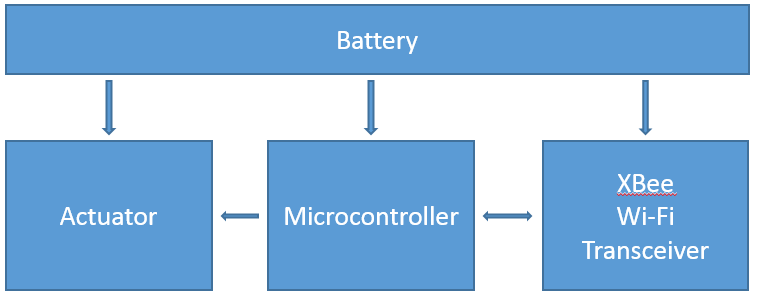
\includegraphics[width=.9\textwidth]{VentCntlDiagram.png}
\caption{Vent Duct Controller component diagram from Fig.~\ref{fig:maindiagram}.}
\label{fig:ventdiagram}
\end{figure}

\subsection{Block Descriptions}
\label{sect:blockdescriptions}
\subsubsection{Overall System Summary}
The overall system will consist of one main control panel, a central HVAC system, and any number of remote temperature sensors and duct vent controllers.  At least one remote temperature sensor is required for the system to be ``smart'', such that it will be able to detect temperatures in rooms other than where the normal thermostat (main control panel) is located.  The duct vent controllers also follow a similar logic, as many duct controllers would be used as desired to control air flow to desired rooms, but at least two are required to make the system work as intended.
%There are several components used in many of the components: temperature and humidity sensors, microcontrollers, and wireless transceivers.
\paragraph{Temperature Sensors}
An LM35 temperature sensor is used to get an accurate reading of temperature in all components. The sensors will be read by the microcontrollers and used along with humidity sensors to determine HVAC on/off state and vents open/closed state.
\paragraph{Humidity Sensors}
An HH10D humidity sensor will be used to measure the relative humidity around the sensor.  The humidity reading will be used along with the temperature reading to set the temperatures in each room.
\paragraph{Central HVAC}
No modifications to a home's central HVAC system is desired.  In the United States, most central HVAC systems supply a $24\, \rm VAC_{RMS}$ power for a thermostat, and receive turn on and off signals from the thermostat.  The main control panel must provide these signals to the HVAC system.
\subsubsection{Main Control Panel}
The main control panel acts as master to all other components.  The main control panel can be broken down into several components as shown in Fig.~\ref{fig:cntldiagram}. The housing for this main panel should be a plastic case similar to standard thermostats.
\paragraph{Main Panel Power Supply}
The power supply must convert the US standard $24\,\rm VAC_{RMS}$ low voltage wiring for most HVAC thermostat controllers into $3.3\,\rm VDC$, as used by the microcontroller and transceiver. The Power supply will be a full-wave rectifier and a switched mode DC-DC converter.
\paragraph{Main Panel Microcontroller}
The microcontroller used will be an MSP430 microcontroller. The microcontroller must send and receive packets over the network via the wireless transceiver, read the temperature and humidity sensors, signal the central HVAC system on or off, and output to an LCD display for debugging and UI purposes. The main control panel will receive broadcast data from all of the remote temperature sensors on the network (including its own sensors). Once the microcontroller receives temperature information from each remote sensor, it determines which vents to open and close and sends data wirelessly to the desired vent controllers. The HVAC is controlled over a 2-3 wire system connected directly to the HVAC over existing house wiring.
\paragraph{XBee Wi-Fi Transceiver}
The Xbee transciever block is the main communication portion of the design.  The transceivers will all be on a wireless network to allow each component to send/receive messages from the main control panel.  Power for the transceiver is 3.3\,VDC and comes from the power supply. The transciever connects to the microcontroller via serial port.


\subsubsection{Remote Temperature Sensors}
A remote temperature sensor consists of a power supply, microcontroller, sensors, and wireless tranceiver as shown in Fig.~\ref{fig:remotediagram}.  Each remote temperature sensor will be identical, and will be housed in a small plastic case and plugged into an AC outlet.
\paragraph{Remote Temperature Sensor Power Supply}
The power source for this component is a standard AC outlet.  Like the main controller, an AC-DC converter is required to convert the 120\,VAC\,(RMS) into the 3.3\,VDC required by the microcontroller and wireless transceiver.  The conversion will be done using a standard ``wall wart'' style power supply.
\paragraph{Remote Temperature Sensor Microcontroller}
Again, the microcontroller for this component is an MSP430. The goal of this microcontroller is to read the sensors and output a message to the main control panel through the wireless device.
\paragraph{Remote Temperature Sensor XBee Transceiver}
The Xbee transceiver is used in the remote sensor to allow communication to the main control panel. It will be connected to the microcontroller via serial port.

\subsubsection{Vent Controllers}
The vent controller, shown in Fig.~\ref{fig:ventdiagram}, will mount inside of a standard HVAC ventilation cover and control the opening and closing of the vent.  Opening and closing of the vent will allow the system control over HVAC flow out of the desired vent, and by extension, the room. The vent controller will receive messages from the main control panel and open or close the vent using an actuator connected to the vent's existing closer. Each vent controller will be identical and can be replicated as desired.
\paragraph{Vent Controller Battery}
Since many homes have vents which are not near AC outlets, and it is not desirable to add a great deal of house wiring, the vent controllers will be battery powered.  9V batteries will be used to supply power to the microcontroller, transceiver, and actuator motor.
\paragraph{Vent Controller Microcontroller}
The MSP430 is used to receive messages from the main control panel via the wireless transceiver.  Once a message is received, the controller will command a small DC actuator to open/close the vent.
\paragraph{Vent Controller XBee Transceiver}
The wireless transceiver in the vent controller will receive only. It will receive messages via the wireless network and forward the message over a serial connection.
\paragraph{Vent Controller Actuator}
The actuator will be a small DC servo motor controlled by the microcontroller.  It will be powered by the 9\,V batteries.  It will operate in two directions and turn a shaft to two positions: $0^\circ$ and $90^\circ$. $0^\circ$ will be the ``Vent OFF'' position and $90^\circ$ will be the ``Vent ON'' position.

